\question A proton traveling in the $-\hat{x}$ direction approaches a capacitor consisting of two large, oppositely charged metal plates. The proton enters the capacitor through a small hole in one of the plates at location $A$ with a speed of $1.6\times10^4\ \mathrm{m/s}$. It exits through a small hole at location $B$ with a speed of $3.9\times10^4\ \mathrm{m/s}$.

\begin{center}
	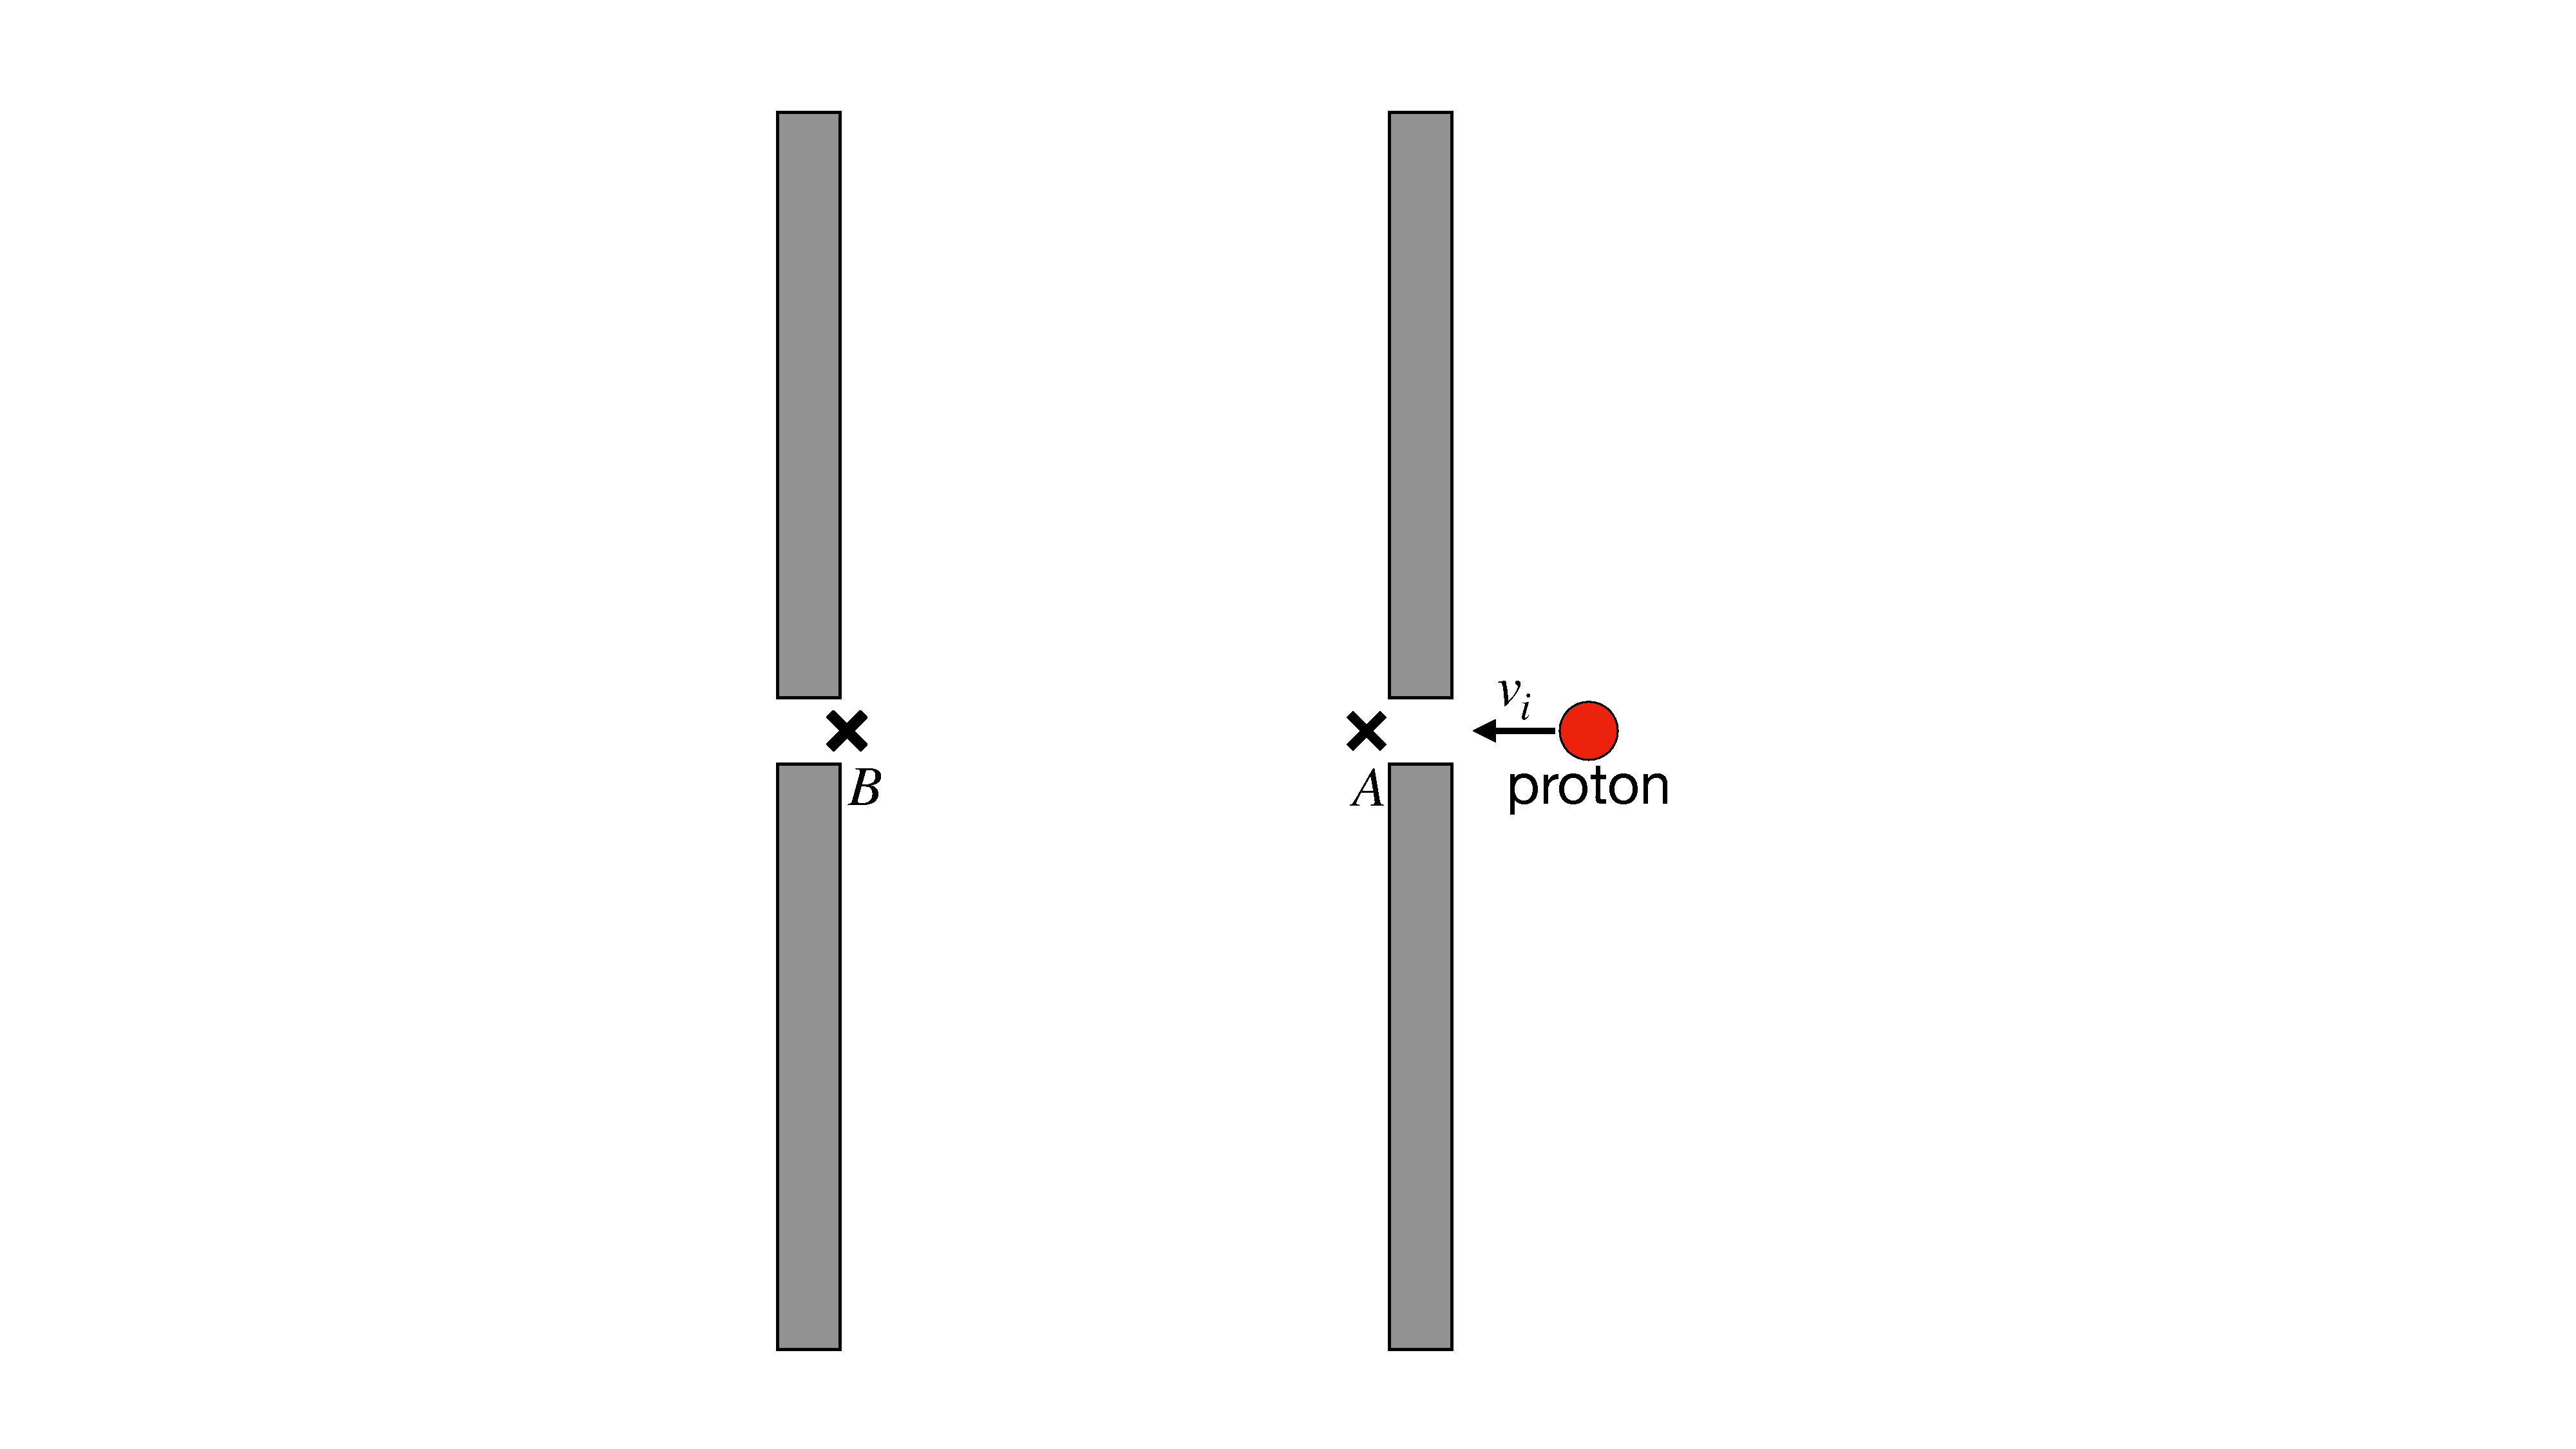
\includegraphics[width=.4\textwidth]{ch16exam.pdf}
\end{center}

\begin{parts}
	\part[5] On the diagram, draw an arrow indicating the direction of the electric field within the gap between the capacitor plates, and indicate which plate is positively charged and which is negatively charged.
	\part[15] What is the potential difference $\Delta V=V_B-V_A$?
\end{parts}